\documentclass{article}

\usepackage{amsthm}
\usepackage{amsfonts}
\usepackage{amsmath}
\usepackage{amssymb}
\usepackage{fullpage}
\usepackage{graphicx}
\usepackage[usenames]{color}
\usepackage{hyperref}
\usepackage{graphicx}

  \hypersetup{
    colorlinks = true,
    urlcolor = blue,       
    linkcolor= blue,      
    citecolor= blue,      
    filecolor= blue,     
    }
    
\usepackage{listings}

\definecolor{dkgreen}{rgb}{0,0.6,0}
\definecolor{gray}{rgb}{0.5,0.5,0.5}
\definecolor{mauve}{rgb}{0.58,0,0.82}

\lstset{frame=tb,
  language=haskell,
  aboveskip=3mm,
  belowskip=3mm,
  showstringspaces=false,
  columns=flexible,
  basicstyle={\small\ttfamily},
  numbers=none,
  numberstyle=\tiny\color{gray},
  keywordstyle=\color{blue},
  commentstyle=\color{dkgreen},
  stringstyle=\color{mauve},
  breaklines=true,
  breakatwhitespace=true,
  tabsize=3
}

\theoremstyle{plain} 
   \newtheorem{theorem}{Theorem}[section]
   \newtheorem{corollary}[theorem]{Corollary}
   \newtheorem{lemma}[theorem]{Lemma}
   \newtheorem{proposition}[theorem]{Proposition}
\theoremstyle{definition}
   \newtheorem{definition}[theorem]{Definition}
   \newtheorem{example}[theorem]{Example}
\theoremstyle{remark}    
  \newtheorem{remark}[theorem]{Remark}

\title{CPSC 354 Report}
\author{Andrew Eppich  \\ Chapman University}
\date{\today}

\begin{document}

\maketitle

\begin{abstract}

\end{abstract}

\tableofcontents

\section{Introduction}\label{intro}

\section{Homework 1}\label{homework1}

\subsection{Question 5}

\begin{lstlisting}
rw [add_zero]
rw [add_zero]
rfl
\end{lstlisting}

\subsubsection{Proof Explanation}

For this question, the Lean proof is related to the corresponding proof in mathematics because we know that we can use the additive identity property, which says that \(x + 0 = x\). By using this, we can simplify \(b + 0\) and \(c + 0\) easily to get \(a + b + c = a + b + c\), which we can determine is the same by the reflexivity property, which states that if \(a = b\), then \(a\) and \(b\) are identical. Therefore, \(a + b + c\) is identical to \(a + b + c\).

\subsection{Question 6}

\begin{lstlisting}
rw [add_zero c]
rw [add_zero b]
rfl
\end{lstlisting}


\subsection{Question 7}

\begin{lstlisting}
rw [one_eq_succ_zero]
rw [add_succ]
rw [add_zero]
rfl
\end{lstlisting}


\subsection{Question 8}

\begin{lstlisting}
rw [two_eq_succ_one]
rw [one_eq_succ_zero]
rw [add_succ]
rw[add_succ]
rw [add_zero]
rw [four_eq_succ_three]
rw [three_eq_succ_two]
rw [two_eq_succ_one]
rw [one_eq_succ_zero]
rfl
\end{lstlisting}

\subsection{Discord Question}

I was wondering if the computers use of discrete math extends to all program computations or just math computations

\section{Homework 2}\label{homework2}

\subsection{Question 1}

\begin{lstlisting}
induction n with d hd
rw [add_zero]
rfl
rw [add_succ]
rw [hd]
rfl
\end{lstlisting}

\subsection{Question 2}

\begin{lstlisting}
  induction b with d hd
  rw [add_zero]
  rw [add_zero]
  rfl
  rw [add_succ]
  rw [add_succ]
  rw [hd]
  rfl
\end{lstlisting}

\subsection{Question 3}

\begin{lstlisting}
induction b with d hd
rw [add_zero]
rw [zero_add]
rfl
rw [add_succ]
rw [hd]
rw [succ_add]
rfl
\end{lstlisting}

\subsection{Question 4}

\begin{lstlisting}
  induction a with d hd
  rw [zero_add]
  rw [zero_add]
  rfl
  rw [succ_add]
  rw [succ_add]
  rw [succ_add]
  rw [hd]
  rfl
\end{lstlisting}

\subsubsection{Explaination}

The lean proof relates to the proof in mathematics because it uses induction to solve the problem. Then the Lean proof is solved by solving the equation of the successors. Just like in mathematics it uses simple rules to change the positioning of the parenthesis so each side is exactly the same. This is exactly like how the mathematical proof would be written.

\subsection{Question 5}

\begin{lstlisting}
  induction a with d hd
  rw [zero_add]
  rw [zero_add]
  rw [add_comm]
  rfl
  rw [add_comm]
  rw [add_comm]
  rw [succ_add]
  rw [succ_add]
  rw [succ_add]
  rw [succ_add]
  rw [hd]
  rfl
\end{lstlisting}

\subsection{Discord Question}

I was wondering how discrete math and the recursive algorithms we talked about fit into a programming language and how it actually works

\section{Homework 3}\label{homework3}

\subsection{Discord Post}

Discord Name: Andrew Eppich.   
In my literature review with ChatGPT, I explored interpreted vs. compiled programming languages. I found that interpreted languages are changed from user to machine code line by line, which is inefficient. Compiled languages are compiled from user to machine code all at once and then run which makes it faster and easier to spot errors. From there I explored interpreted languages and their role in machine learning as well as their history in machine learning. I first found that compiled was much more efficient than interpreted. I then found out that interpreted is mainly used for machine learning. It is mainly used because of the extensive amount of libraries used with interpreted languages, especially Python. Some of those libraries include NumPy, pandas, scikit-learn, TensorFlow, and Matplotlib. These libraries are crucial for machine learning because they are associated with data processing and deep learning. I then took a look into the history of programming languages with machine learning. I found that at first compiled languages were used from the 1950s-1980s. In 1991, Python was developed which became the standard for machine learning in the early 2000s. Python became the main language for machine learning from 2010 and on because of its libraries TensorFlow and PyTorch. 
\url{https://github.com/AndrewEppich/LLM-Literature-Review/blob/main/README.md}

\subsection{Reports Voted For}

\url{https://github.com/zackklopukh/LLMReport}

\url{https://github.com/maxler0y/354_HW3}

\section{Homework 4}\label{homework4}

\begin{figure}[h]
  \centering
  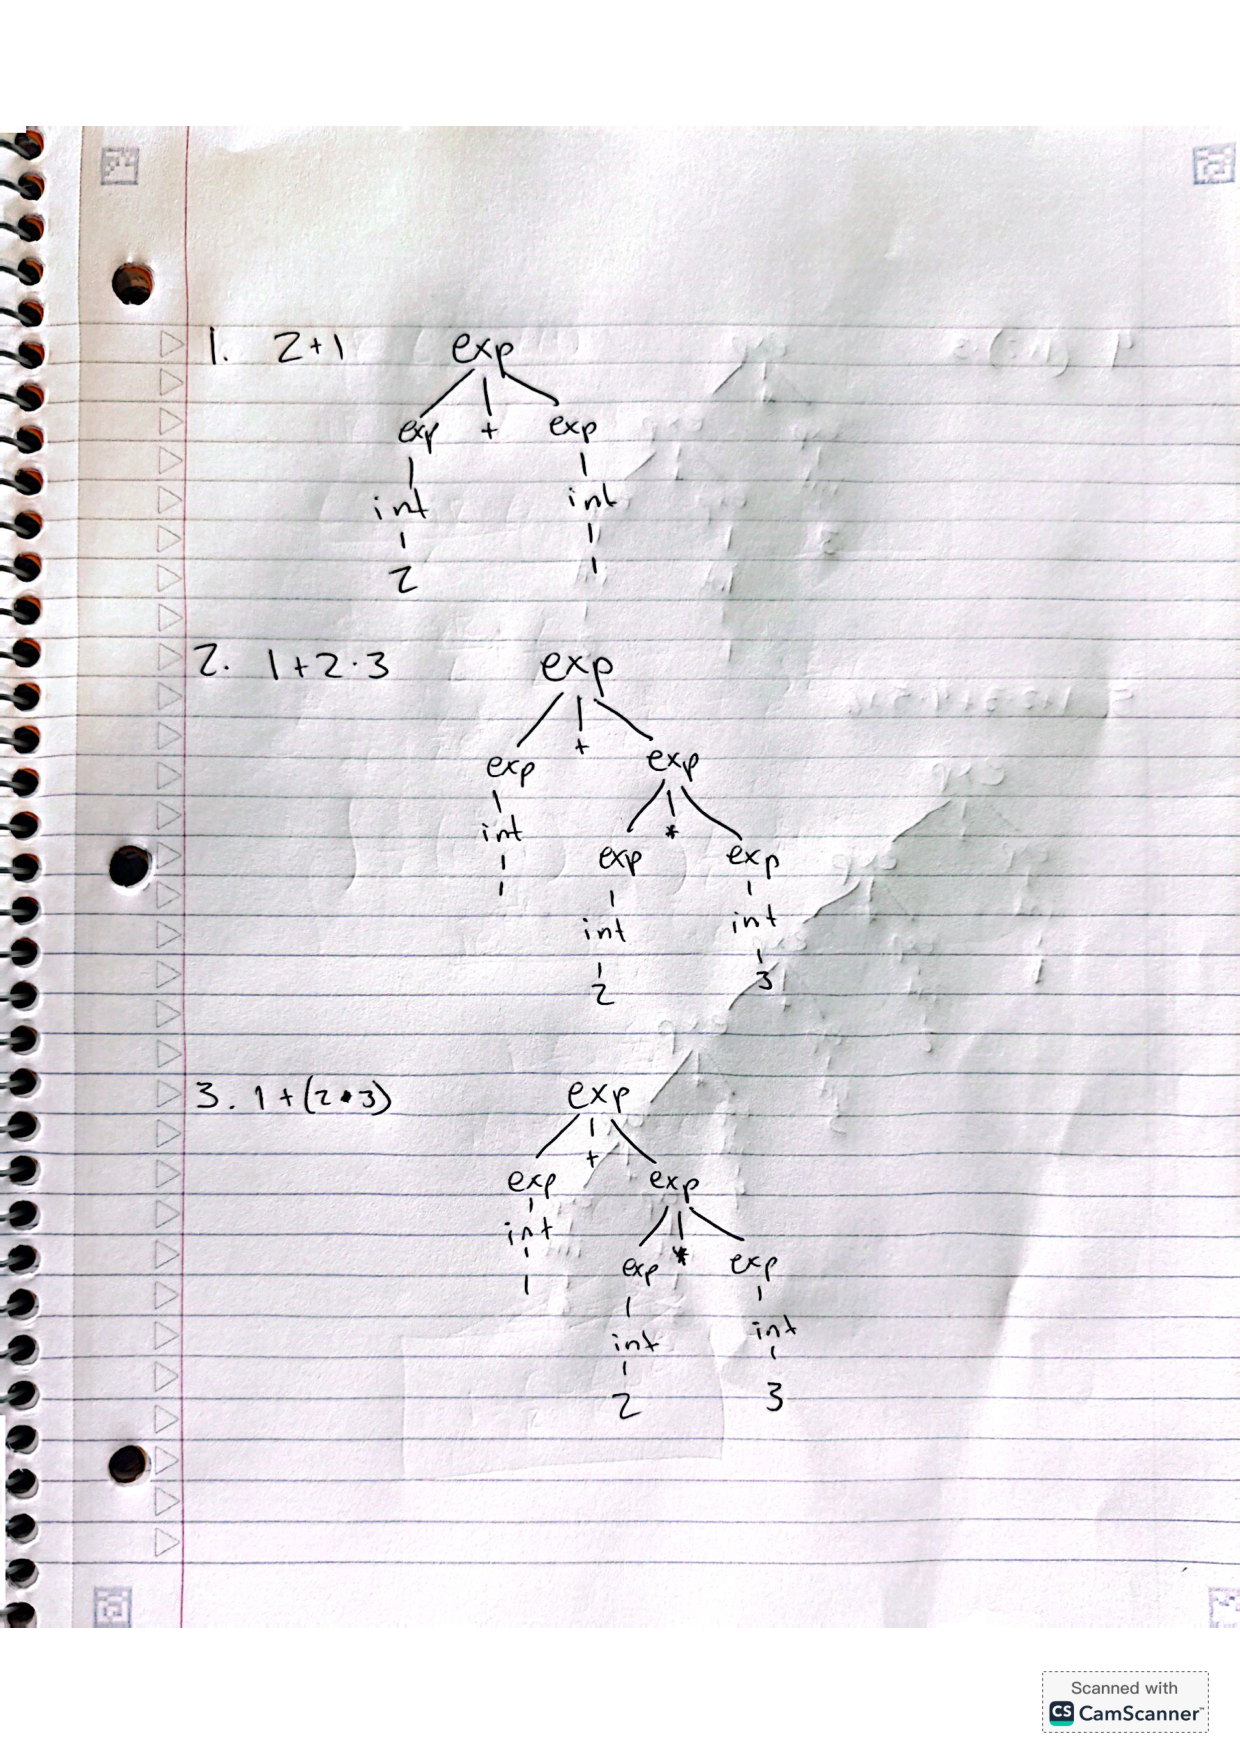
\includegraphics[width=0.7\textwidth, page=1]{CPSC_354_Homework_4.pdf}
  \label{fig:sample_pdf}
\end{figure}

\begin{figure}[h]
  \centering
  \includegraphics[width=0.7\textwidth, page=2]{CPSC_354_Homework_4.pdf}
  \label{fig:sample_pdf}
\end{figure}

\subsection{Discord Question}

How complex do parsing algorithms get the farther down the level of programming languages you go?


\section{Homework 5}\label{homework5}

\subsection{Question 1}

\begin{lstlisting}
  exact todo_list
\end{lstlisting}

\subsection{Question 2}

\begin{lstlisting}
  exact and_intro p s
\end{lstlisting}

\subsection{Question 3}

\begin{lstlisting}
  exact ⟨⟨a,i⟩,⟨o,u⟩⟩
\end{lstlisting}

\subsection{Question 4}

\begin{lstlisting}
  have p := vm.left
  exact p
\end{lstlisting}

\subsection{Question 5}

\begin{lstlisting}
  exact and_right h
\end{lstlisting}

\subsection{Question 6}

\begin{lstlisting}
  have a:= and_left h1
  have b := and_right h2
  exact ⟨a, b⟩
\end{lstlisting}

\subsection{Question 7}

\begin{lstlisting}
  have h1 := h.right
  have h2 := h.left
  have h3 := h2.right
  exact h.left.right.left.left.right
\end{lstlisting}

\subsection{Question 8}

\begin{lstlisting}
  have h1 := and_left h
  have h2 := and_right h
  have h3 := and_right h2
  have h4 := and_left h3
  have h5 := and_left h4
  have h6 := and_right h1
  have h7 := and_left h1
  have h8 := and_left h7
  have h9 := and_right h7
  exact ⟨h6, h5, h8, h9⟩
\end{lstlisting}

\subsection{Discord Question}

\end{document}
